\subsection{Cas continu}

La résolution de \emph{MountainCar continuous} rencontre un obstacle:
l'acquisition de la récompense. En effet, l'agent est pénalisé à chaque pas qu'il effectue. C'est uniquement lorsqu'il atteint son but qu'il recoit une récompense conséquente de \(100\) points. Le problème donc d'arriver effectivment à ce but.

\begin{figure}[htb]
    \centering
    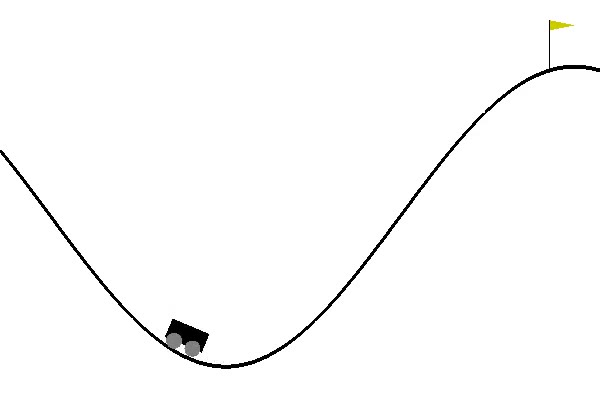
\includegraphics[width=0.5\textwidth]{figures/mountain_car/env.jpeg}
    \caption{Représentation graphique du problème MountainCar-V0}
    \label{fig:mountain_car_continuous}
\end{figure}

Le domaine des actions du système ne lui permet pas de gravir directement la pente qui le sépare de son objectif. Il doit dans un premier temps prendre un léger élan devant pour gagner en vitesse et arriver assez haut sur la pente derrière lui. Avec la hauteur accumulée, en poussant finalement à droite, il aura accumuler assez de vitesse pour atteindre le but. Cette séquence d'action bien précise est presque impossible à obtenir avec de l'exploration simple. C'est pourquoi il est conseillé d'utiliser un \emph{politique experte}. 

Le rôle de cette politique experte est d'atteindre le but sans apprentissage. Elle va être codée de façon à reproduire ce qu'on pense être un comportement optimal. Nous la faisons réaliser plusieurs trajectoires que nous enregistrons dans le \emph{replay buffer} de notre simulation. Nous pouvons ainsi entraîner notre politique et nos critiques du \emph{Soft Actor Critic} sur ces trajectoires majoritairement satisfaisantes.

Finalement, nous pouvons lancer l'apprentissage du \emph{Soft Actor Critic} comme pour le problème du \emph{Pendulum} mais avec une politique et des critiques déjà pré-entraînées.

\begin{figure}[H]
    \centering
    \begin{subfigure}{0.45\textwidth}
        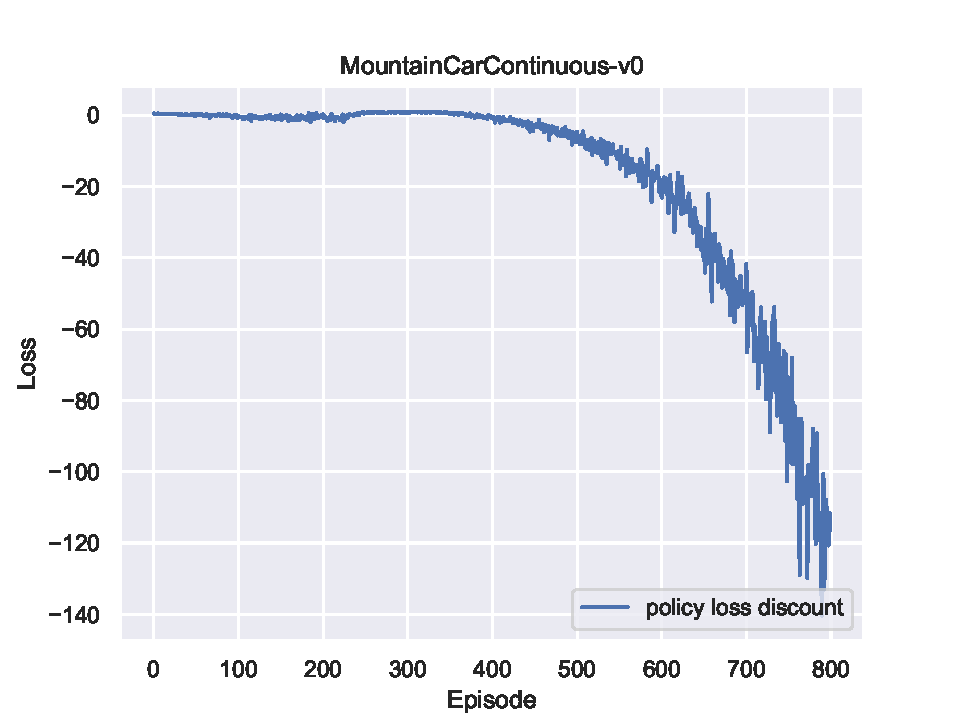
\includegraphics[width=\textwidth]{figures/mountain_car/policy_loss_MountainCarContinuous-v0_pg_dataset_td_trajs_800_update_threshold_1000_nb_updates_20_gamma_0.98_tau_0.01_nstep_5_lr_act_0.0005_lr_critic_0.001_init_alpha_0.02_lr_alpha_0.0_target_entropy_alpha_-1.0pg.pdf}
        \caption{Fonction de perte de la politique}\label{fig:mountain:policy_loss}
    \end{subfigure}
    \begin{subfigure}{0.45\textwidth}
        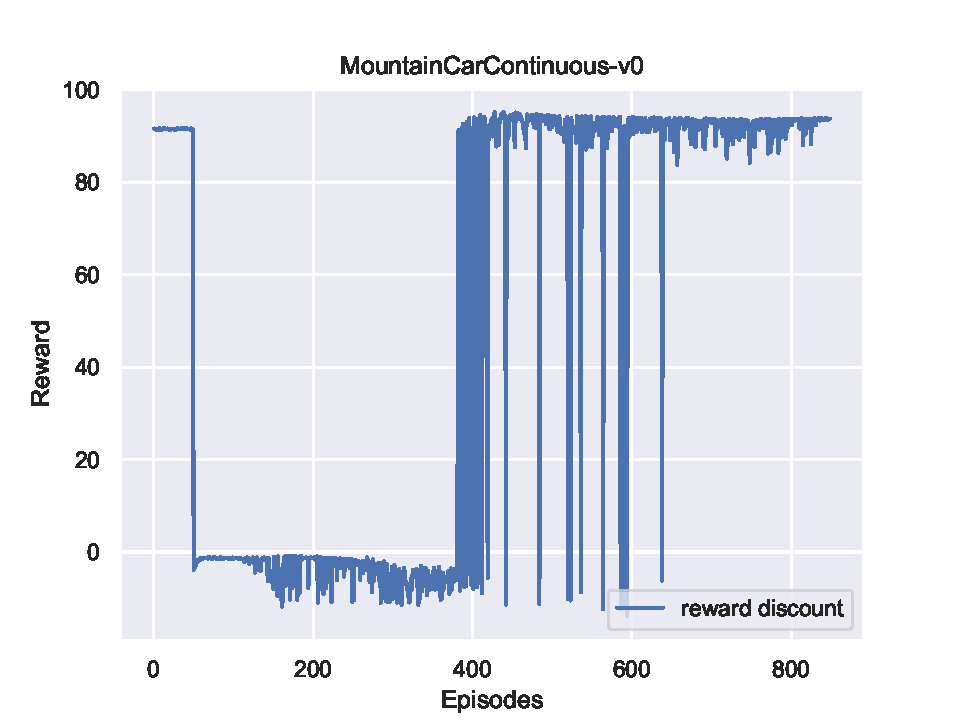
\includegraphics[width=\textwidth]{figures/mountain_car/rewards_MountainCarContinuous-v0_pg_dataset_td_trajs_800_update_threshold_1000_nb_updates_20_gamma_0.98_tau_0.01_nstep_5_lr_act_0.0005_lr_critic_0.001_init_alpha_0.02_lr_alpha_0.0_target_entropy_alpha_-1.0.pdf}
        \caption{Récompenses}\label{fig:mountain:reward}
    \end{subfigure}
    \begin{subfigure}{0.45\textwidth}
        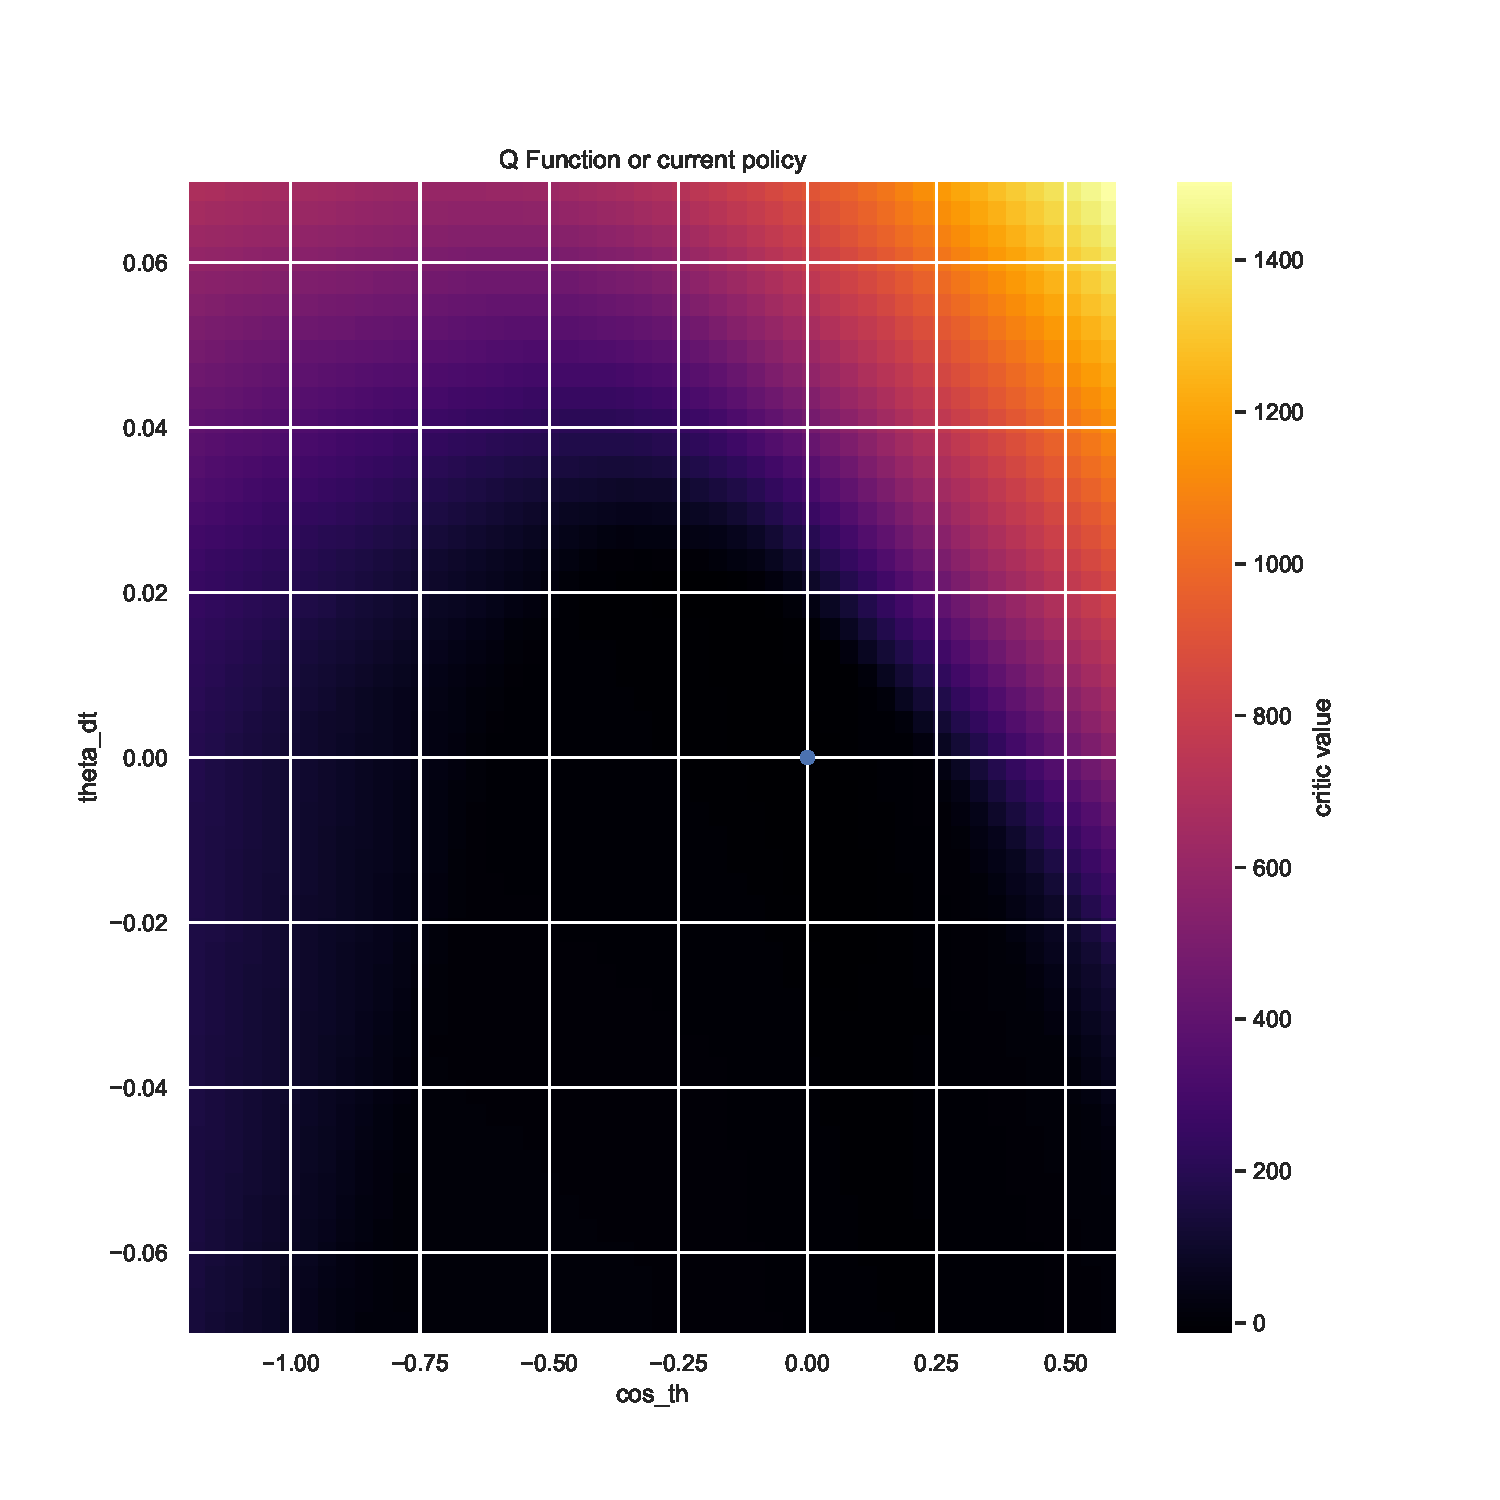
\includegraphics[width=\textwidth]{figures/mountain_car/0_critic_pg_q1_post_MountainCarContinuous-v0.pdf}
        \caption{Critique obtenue après entraînement. L'abscisse correspond à la position de l'agent et l'ordonnée correspond à se vitesse.}\label{fig:mountain:critic}
    \end{subfigure}
\end{figure}

Nous pouvons constater sur la figure des récompenses (fig~\ref{fig:mountain:reward}) qu'au début, l'agent cherche l'objectif sans le trouver. Cela donne toujours le même récompense. Quand il trouve enfin le but, la croissance de la récompense est drirecte et la fonction de perte de la politique (fig~\ref{fig:mountain:policy_loss}) décroit dortement.

Enfin nous pouvons voir sur la critique (fig~\ref{fig:mountain:critic}) que l'apprentisage favorise effectivement la position où se trouve l'objectif. C'est à dire tout à droite uniquement obtenable avec une vitesse positive assez élevée.